\documentclass{standalone}
\usepackage{tikz}

\begin{document}
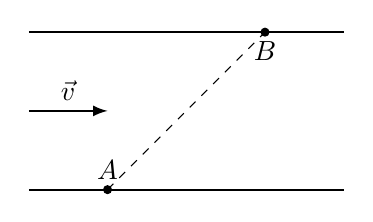
\begin{tikzpicture}    
	\draw [thick] (0,2) -- (4,2);
	\draw [thick] (0,0) -- (4,0);
	\draw [arrows={-latex}, thick] (0, 1) -- (1, 1) node [above, midway] {$\vec{v}$};
	\draw [dashed] (1,0) -- (3,2); 
	\draw [fill] (1,0) circle (0.05) node [above] {$A$};
	\draw [fill] (3,2) circle (0.05) node [below] {$B$};
	
\end{tikzpicture}
\end{document}